\chapter*{Appendices}
\addcontentsline{toc}{chapter}{Appendices}
\setcounter{section}{0}
\setcounter{figure}{0}
\setcounter{table}{0}
\renewcommand{\thesection}{A.\arabic{section}}
\renewcommand{\thefigure}{A.\arabic{figure}}
\renewcommand{\thetable}{A.\arabic{table}}

\section{Build and Run Notes}

The repository documents separate frontend and backend setup processes. A representative local workflow is shown below.

\begin{lstlisting}[style=thesiscode]
cd backend
npm install
npm run prisma:migrate
npm run dev
\end{lstlisting}

\begin{lstlisting}[style=thesiscode]
cd frontend
npm install
npm run dev
\end{lstlisting}

\section{Selected Environment Variables}

\begin{table}[H]
\centering
\caption{Representative environment variables}
\label{tab:env-vars}
\begin{tabularx}{\textwidth}{L{0.34\textwidth}Y}
\toprule
\textbf{Variable} & \textbf{Purpose} \\
\midrule
\code{NEXT\_PUBLIC\_API\_URL} & Browser-visible API base URL for the frontend. \\
\code{INTERNAL\_API\_URL} & Server-side fetch base used by the frontend runtime. \\
\code{BACKEND\_URL} & Optional rewrite target for same-origin frontend calls. \\
\code{SERVER\_PORT} & Backend listening port. \\
\code{DATABASE\_URL} & PostgreSQL connection string for Prisma. \\
\code{JWT\_SECRET} & Secret used to verify and sign JWT tokens. \\
\code{CORS\_ORIGINS} & Allowed origins for cross-origin backend requests. \\
\code{AUTO\_SEED\_ACHIEVEMENTS} & Controls automatic achievement seeding on startup. \\
\bottomrule
\end{tabularx}
\end{table}

\section{Application User Interface Screenshots}

The following pages illustrate the key user interfaces of the Anhoc platform, captured during live local execution of both student and administrative portals.

\begin{figure}[H]
    \centering
    \begin{minipage}{0.48\textwidth}
        \centering
        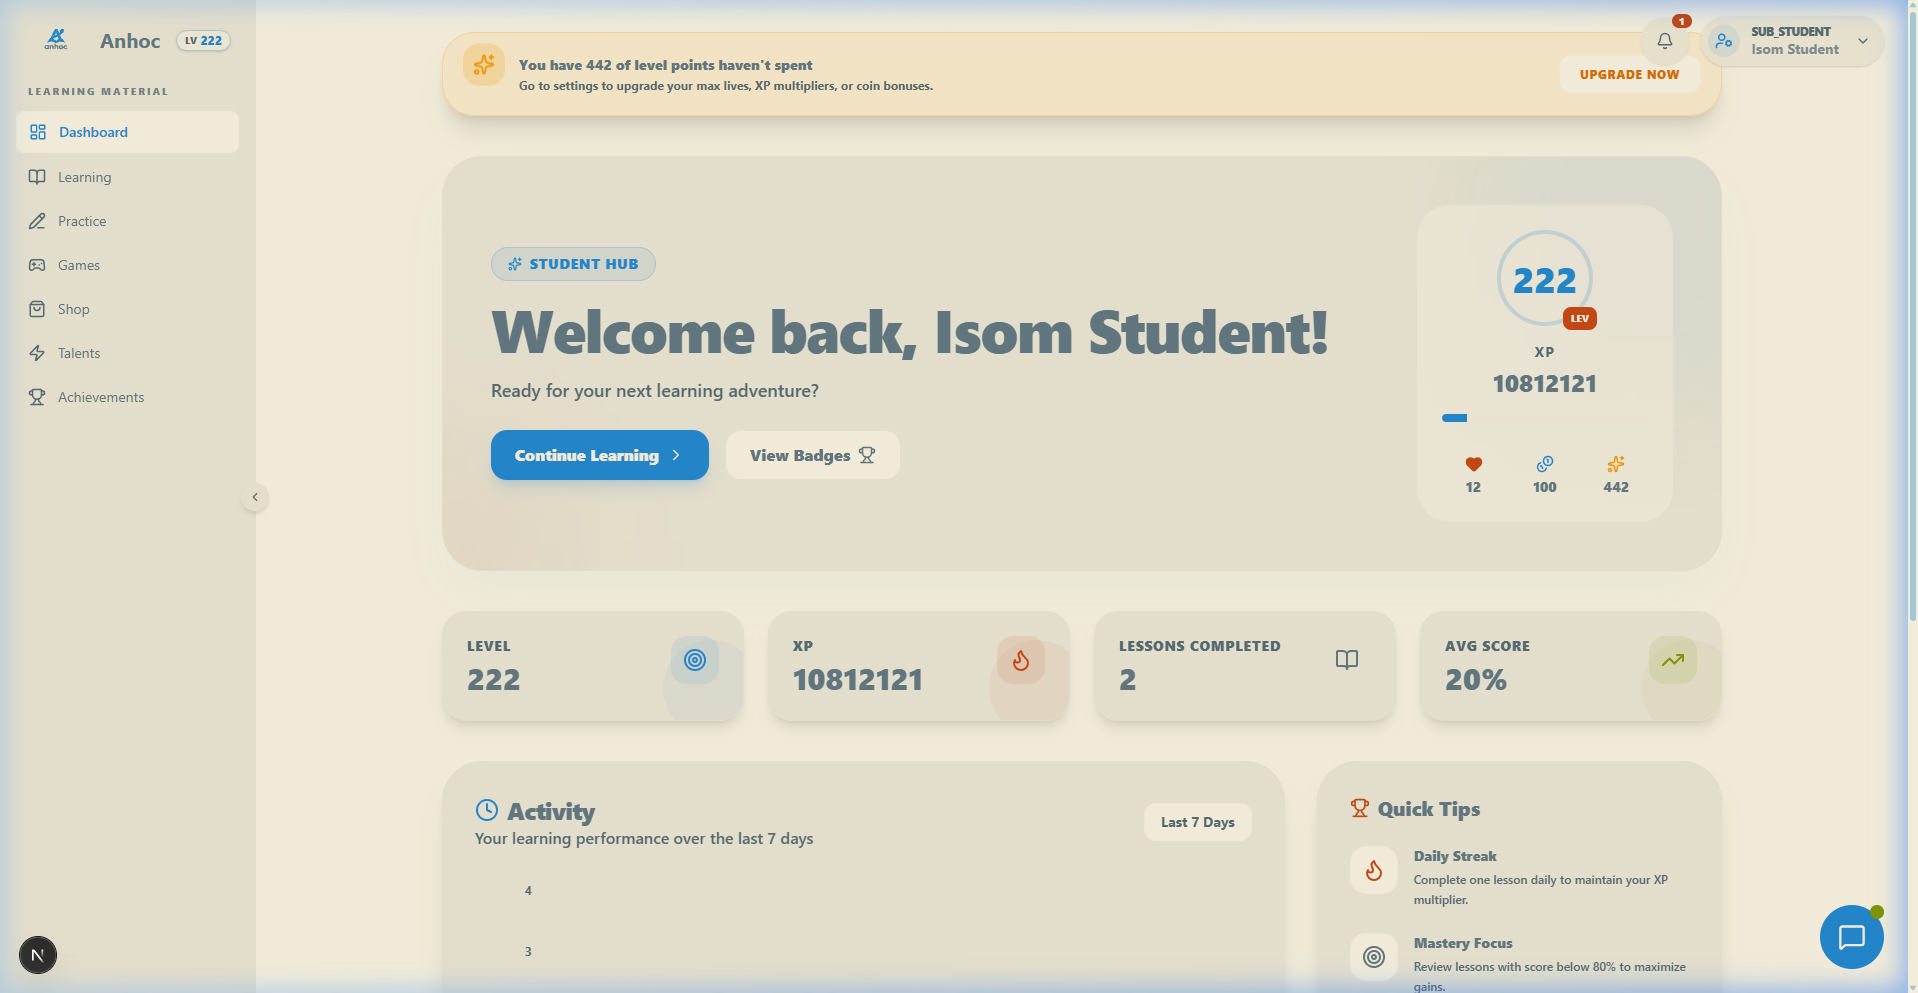
\includegraphics[width=\textwidth]{images/student_dashboard.png}
        \caption{Student dashboard showing XP, levels, and achievements.}
        \label{fig:student_dashboard}
    \end{minipage}
    \hfill
    \begin{minipage}{0.48\textwidth}
        \centering
        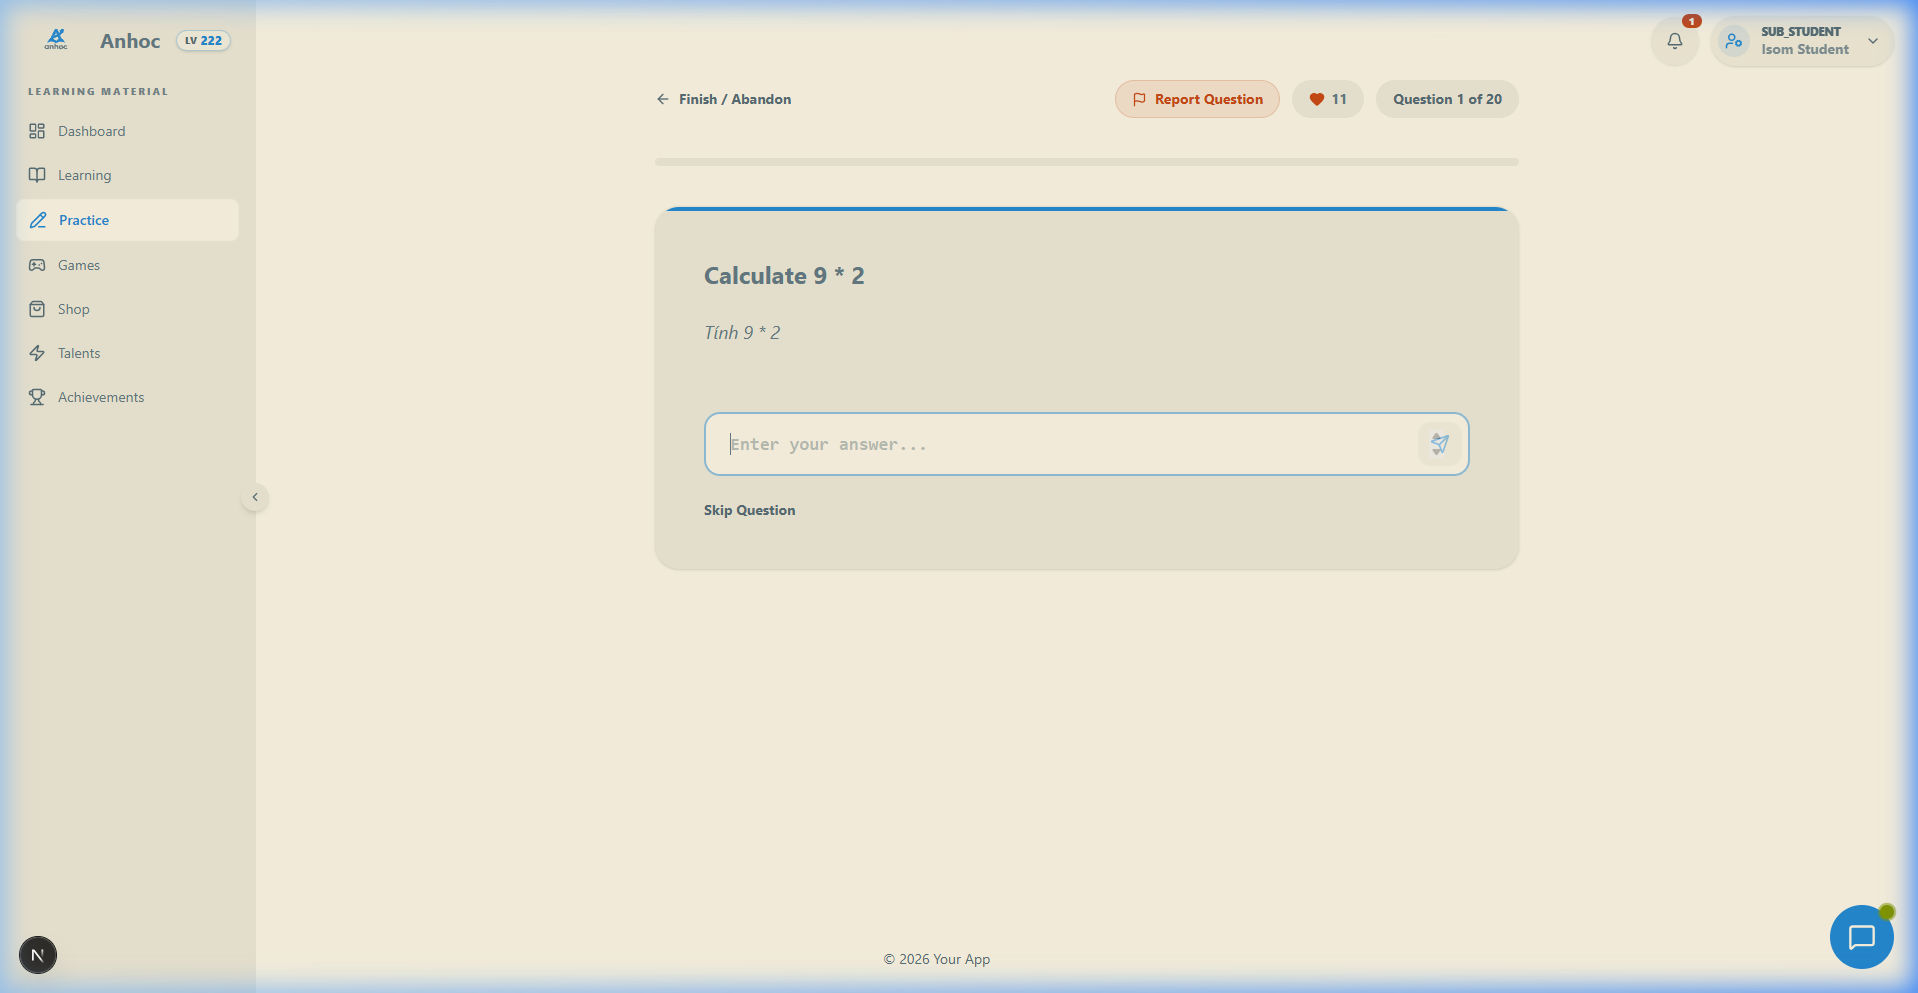
\includegraphics[width=\textwidth]{images/lesson_practice.png}
        \caption{Interactive mathematics practice interface.}
        \label{fig:lesson_practice}
    \end{minipage}
\end{figure}

\begin{figure}[H]
    \centering
    \begin{minipage}{0.48\textwidth}
        \centering
        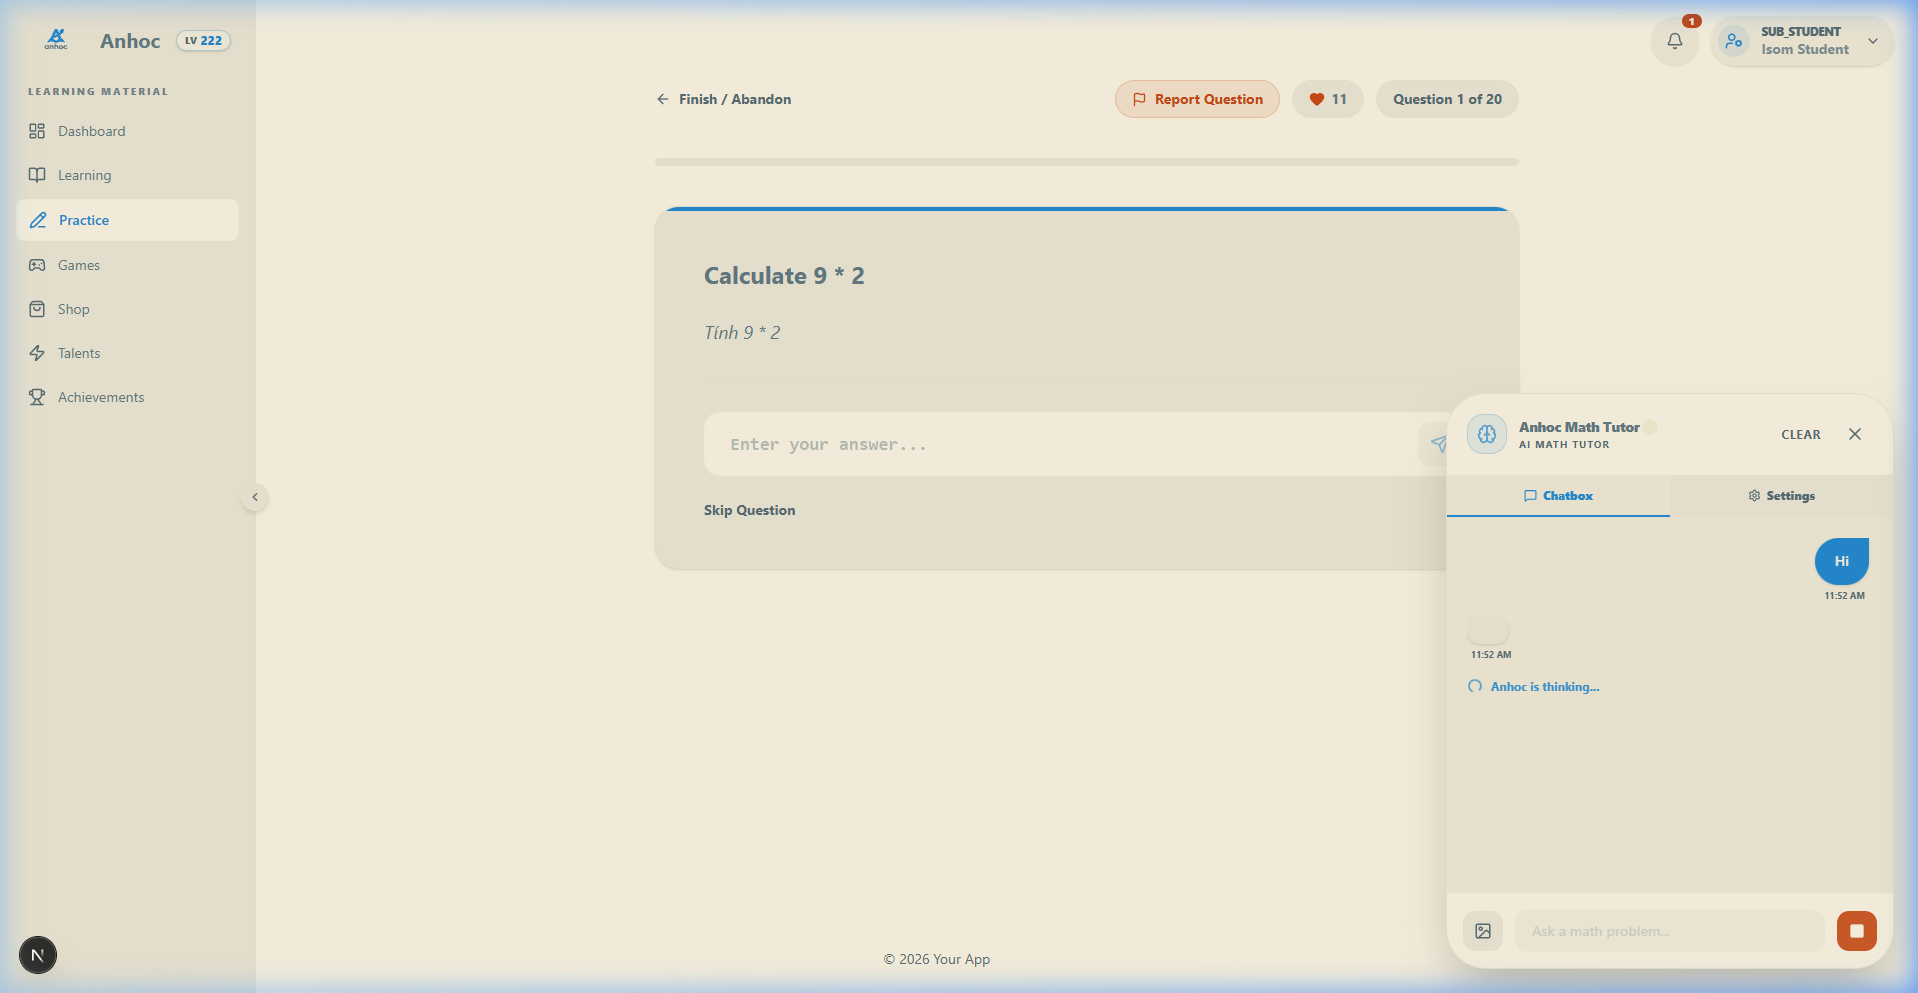
\includegraphics[width=\textwidth]{images/chatbot_widget.png}
        \caption{AI tutoring chatbot widget with reasoning.}
        \label{fig:chatbot_widget}
    \end{minipage}
    \hfill
    \begin{minipage}{0.48\textwidth}
        \centering
        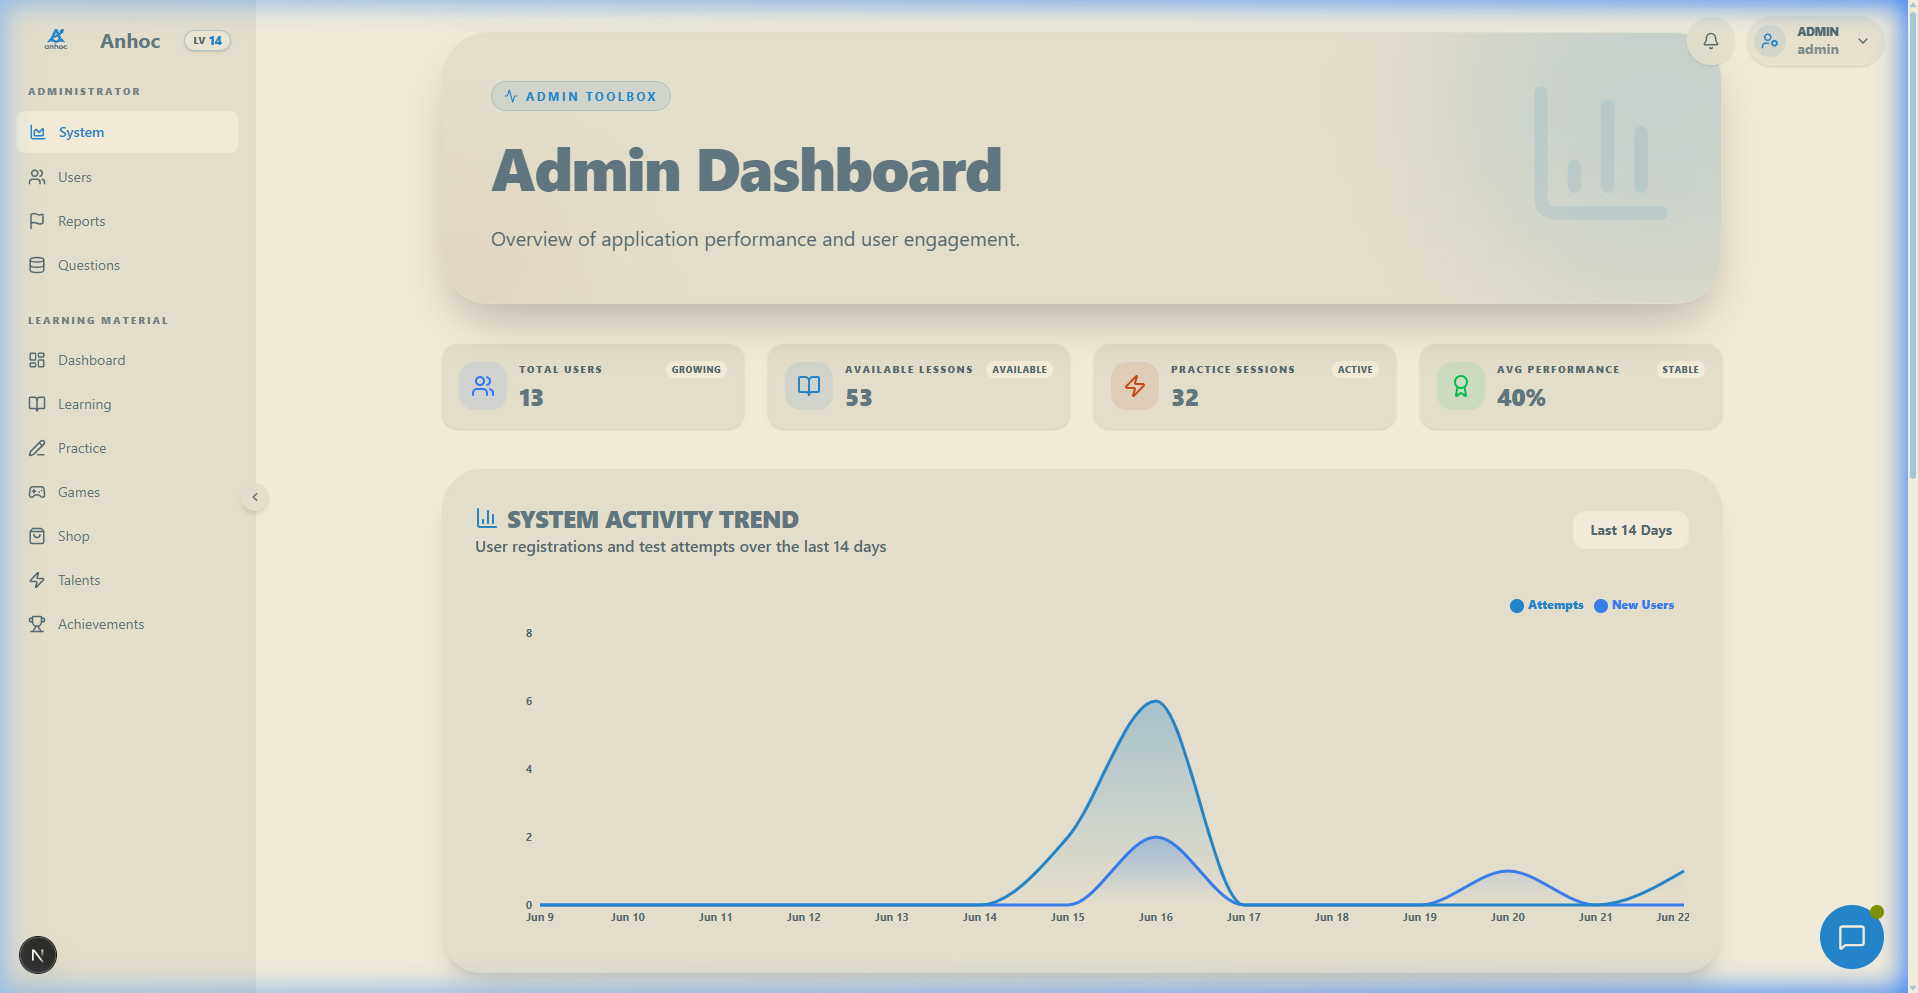
\includegraphics[width=\textwidth]{images/admin_dashboard.png}
        \caption{Administrative overview panel.}
        \label{fig:admin_dashboard}
    \end{minipage}
\end{figure}

